%[How did it go as an application to robotics? does it make sense? performance? tests? comparisons to other communication forms?]
\todo{what requirements? what is good communication for the robot?}

After all the due measurements and evaluations of the prototype from purely a communication point of view, the system was tested in the context of mobile robotics.
To evaluate the system in regards to its intended applicative scenario, a small mobile robot was equipped with a receiver module from the prototype and a Raspberry Pi to receive the information, implement the logical layer of the receiver and control the robot movements accordingly.
 Different experiments were conducted, to test the functionalities of the communication as a generic communication system, and to exploit the property of the light as a situated medium of communication.

%setup
\subsection{Experimental setup}
For this evaluation the receiver has been mounted on top of a Thymio-II \cite{thymio}, a small educational robot developed  by MOBOTS, a group of the Swiss Federal Institute of Technology in Lausanne (EPFL), in collaboration with the Lausanne Arts School (ECAL).
The receiver's sensor has been placed to face in the same direction that the front of the robot faces.
The receiver board has been connected to a Raspberry Pi \cite{raspberrypi}, also mounted on top of the robot.
The Raspberry Pi provides enough computational power to implement the logical layer of the system (section \ref{logical}), and it also offers the full capabilities of controlling the Thymio robot.
Raspberry Pi and Thymio have been connected through a serial connection with a USB cable.
For the transmitter the same previous setup has been kept, with an Arduino board controlling a low power super bright LED, receiving input from a computer that takes user input.

%components
\subsubsection{List of components}
\begin{enumerate}
\item Photoconductive Cell VT900
\item Genuino Yun micro controller board, based on ATmega32u4 \cite{arduinoyun}
\item Raspberry Pi 3 Model B to be applied on a mobile robot
\item Thymio-II educational robot
\end{enumerate}

\subsubsection{Wiring}
\todo{diagram with connections for experiment with robot}

%experiments
\subsection{Experiments}
The \textbf{first experiment} that has been performed was to test the overall capabilities of the communication system with the new setup.
The experiments merely consisted of transmitting movement instructions like any common remote control.
The commands tested were: forward, backwards, left, right and stop.
Commands were taken from user input on the computer controlling the transmitter, and transmitted through light.
Upon reception, the receiver would then control the robot movements accordingly.
\newline
A \textbf{second experiment} was conducted to exploit the property of this communication system of being situated and simultaneously its potential to virtually send any message, not only preprogrammed commands.
In this experiment, two more photoresistors were connected to the receiver module, and their values forwarded alongside the one used for reading the signal.
The three sensors are all placed facing forward in regards to the robot's direction, with the central one facing forward and the two on the sides in diagonal to get a view of the sides.
Figure \ref{fig:thymioangles} shows the placement of the sensors graphically.

\begin{figure}[hbt]
\centering
  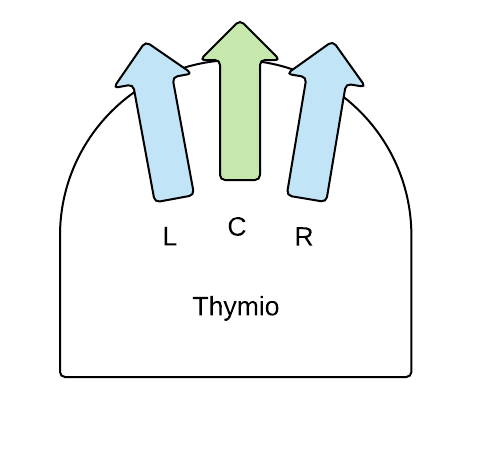
\includegraphics[height=100px]{img/thymioangles}
  \caption{Placement of the sensors in front of the robot, only the central one reads communication, while the ones on the sides help direction.}
  \label{fig:thymioangles}
\end{figure}
%
The robot is programmed to always face the light source, and turn to the side whose sensor registers more light, above a certain limit.
The experiment consists of reprogramming the robot's behaviour based on the message sent encoded in light.
When the message instructs to approach the light source, the robot actively follows the light source moving forward.
When the message instructs to move away from the light source, the robot moves backwards away from the light source, still facing its direction.
This is an example of messages that potentially reprogram the behaviour of the agent, adding as a plus information about relative position of the source of the message.
To distinguish this case from a case of preprogrammed reactions to specified commands, the message contains the velocity parameter that the robot needs to apply to its motors, instead of merely say 'forward' and 'backwards' like in the previous experiment.
When the velocity is positive, the robot approaches the light source, following it and moving forward, when the velocity is negative the robot will evade the light source moving backwards away from it.
Depending on the specific value contained in the message, the robot will move at different speeds.\\

This experiment is intended to demonstrate that a communication system that allows generic communication can be used to transmit a wide range of complex instructions, represented in this experiment as a wide range of potential values for the same parameter, velocity in this case.
The fact that the system exploits a form of situated communication adds to the message the information of direction and positioning relative to the source of the message.
Rather than programming a robot to present a behaviour in reaction to a predetermined command, the experiment directly instructs the robot to exhibit the new behaviour, represented by a velocity of custom intensity and direction.
Therefore, the behaviour is not known to the robot beforehand, but is dynamically received and executed.
This way of communicating instructions can arguably produce an infinite range of possible outcomes.
On the other hand encoding predetermined commands into finite sets of signals could result limiting in certain applications.
Dynamic instructions could prove decisive in applications where behaviours need to be adjusted depending on variable circumstances, or where the set of instructions is just too big to be mapped to distinct signals within a reasonable effort.

The same effect could be achieved by a system that uses two separate communication subsystems, one reactive and situated, like a coloured light or an infrared sensor, and another generic and local, like could be Bluetooth.
If two agents have the ability to identify each other, generic communication could be exchanged through any wireless medium, like WiFi.
A visible light communication approach however would reduce complexity and achieve the same result, provided that the performance is considered sufficient.

When running the experiments initially, the transmission rate adopted was the one with 2ms duration of each symbol.
This led to poor results and bad reception over distances greater than 10 cm, and was later changed.
The final transmission rate that was chosen was half that, at 4ms duration for each symbol.

%results
\subsection{Performance and Results}

The two experiments were evaluated separately in terms of quality of reception and success rate.
Factors that influence the outcome of the experiments are also taken into account, like distance, angle and interference.

\subsubsection{Remote control}
For this experiments, the system has been tested and evaluated as a generic communication  medium to perform remote control of the robot.
A restricted set of commands is known to the receiver, that has been preprogrammed to react to each of them in a distinct way.
The commands represent movement instructions.
Table \ref{tab:remotectrl} shows the results of these experiments in the best experimental conditions and with a transmission rate of 250 Hz (4 ms intervals).
\begin{table}[hbt]
\centering
  \begin{tabular}{l c c c}
    distance & angle & interference & success rate \\
    \hline
   0-10 cm & direct ($< 15^{\circ}$) & low & 50\%\\
   10-20 cm & direct ($< 15^{\circ}$) & low & 20\%\\
   20-30 cm & direct ($< 15^{\circ}$) & low & $5\%$\\
  \end{tabular}
  \caption{Results of the remote control experiment.}
  \label{tab:remotectrl}
\end{table}
Experimentally, the system appears very sensitive to the exposure to the light source, in terms of angle and facing direction.
The LED used for these experiments has a limited viewing angle of nominally $30^{\circ}$, but the sensor needs to face the centre of the light source to receive the signal correctly.
Facing other directions will greatly reduce the chances of success, even with low deviations.

An effort to slightly increase the success rate with selected commands can be done by comparing a received signal to the possible known outcomes, when the signal is incomplete or wrong.
By computing the edit distance between what has been received and what is expected, the known command more similar to the received message can also be the most likely.
This technique could improve the success rate at the cost of a higher computational burden.
An ideal condition to optimise it's effectiveness is the use of possibly short commands from a restricted set, and fairly distinct to one another.

\subsubsection{Situated dynamic behaviour experiment}
This experiment is composed of two distinct parts, that need to be merged together to obtain the final outcome.
First, the reception process need to be adjusted to take values from multiple light sensors instead of just one, and to control the robot so that it always faces the direction with the higher brightness intensity registered.
Second, specific instructions need to be sent as messages, so that the robot doesn't have any knowledge of commands or behaviours beforehand, but executes the commands as they come in form of messages.
Finally, combining the two parts, the robot will have one behaviour preprogrammed, that is to face the light source, and one dynamically set through the message sent to it, that is how to act in relation to the light source.

The first part might represent a bigger challenge than it might seem.
Taking analog input from one source can be a computationally demanding process since it can slow down the clock rate significantly due to the analog-to-digital conversion process.
Reading analog input from three different sources though is exactly three times slower than reading only from one source.
The accuracy of the new transmission rate is therefore scaled with the reception rate.
With a reception rate of 1200 Hz, a transmission rate of 250 Hz (4 ms intervals) is highly accurate in close proximity, and more robust to distance than faster rates.
With three sensors however, the reception rate drops to 400 Hz, three times slower than before.
This new reception rate brings down the accuracy of transmission.
Where before the transmission of a single symbol could be registered as a sequence of about 5 values from the sensor (1200 values per second means 1.2 values per millisecond, which results in 4.8 values for 4 ms), with the new rate each symbol is only about 2 values long.
This brings the precision of the new setup between the ones from the 1000 Hz and 500 Hz rates of the previous setup with only one sensor.
Therefore, it's plausible to expect a drastic drop in accuracy with this setup.

The second part of the experiment has virtually no real difference with the first experiment, since the system allows the exchange of generic binary data that can represent virtually anything.
The only adjustment that needs to be made is to send parameters instead of commands, and how the receiver responds to them.
%
\todo{how many experiments? how was the placement?}
%
\newline
\begin{table}[hbt]
\centering
  \begin{tabular}{l c c c |}
  distance & angle & interference & success rate\\
    \hline
    0-20 cm & $90^{\circ}$ & no & 10/10\\
    0-20 cm &  $180^{\circ}$ & no & 10/10\\
   20-40 cm &  $90^{\circ}$ & no &10/10 \\
   20-40 cm &  $180^{\circ}$ & no &10/10 \\
   40-60 cm &  $90^{\circ}$ & no & 10/10\\
   40-60 cm &  $180^{\circ}$ & no & 10/10\\
   60-80 cm &  $90^{\circ}$ & no & 10/10\\
   60-80 cm &  $180^{\circ}$ & no & 10/10\\
  80-100 cm &  $90^{\circ}$ & no & 10/10\\
  80-100 cm &  $180^{\circ}$ & no & 10/10\\
  \end{tabular}
  \begin{tabular}{| l c c c}
   distance & angle & interference & success rate\\
    \hline
    0-20 cm & $90^{\circ}$ & yes & 10/10\\
    0-20 cm &  $180^{\circ}$ & yes & 10/10\\
   20-40 cm &  $90^{\circ}$ & yes &10/10 \\
   20-40 cm &  $180^{\circ}$ & yes &10/10 \\
   40-60 cm &  $90^{\circ}$ & yes & 10/10\\
   40-60 cm &  $180^{\circ}$ & yes & 10/10\\
   60-80 cm &  $90^{\circ}$ & yes & 10/10\\
   60-80 cm &  $180^{\circ}$ & yes & 10/10\\
  80-100 cm &  $90^{\circ}$ & yes & 8/10\\
  80-100 cm &  $180^{\circ}$ & yes & 7/10\\
  \end{tabular}
  \caption{Results for robot turning towards the light source, with and without interference.}
  \label{tab:turning}
\end{table}

Table \ref{tab:turning} shows the results of the behaviour of the robot to turn towards the light source.
As can be seen, this first part of the experiment had a high success rate within a close range to the light source.
At longer distances however, the light becomes harder to spot, especially with interference from other sources.
In a dark environment, the presence of reflecting surfaces close to the robot can cause a reflection to be interpreted as the source of the light, where the robot can get stuck if the actual source is not in sight.
An important result of this test is that the light source can be seen from much farther away than the distance necessary for actual communication, making it possible for a robot to approach the source of transmission and enhance the chances of a successful communication.

\begin{figure}[hbt]
\centering
  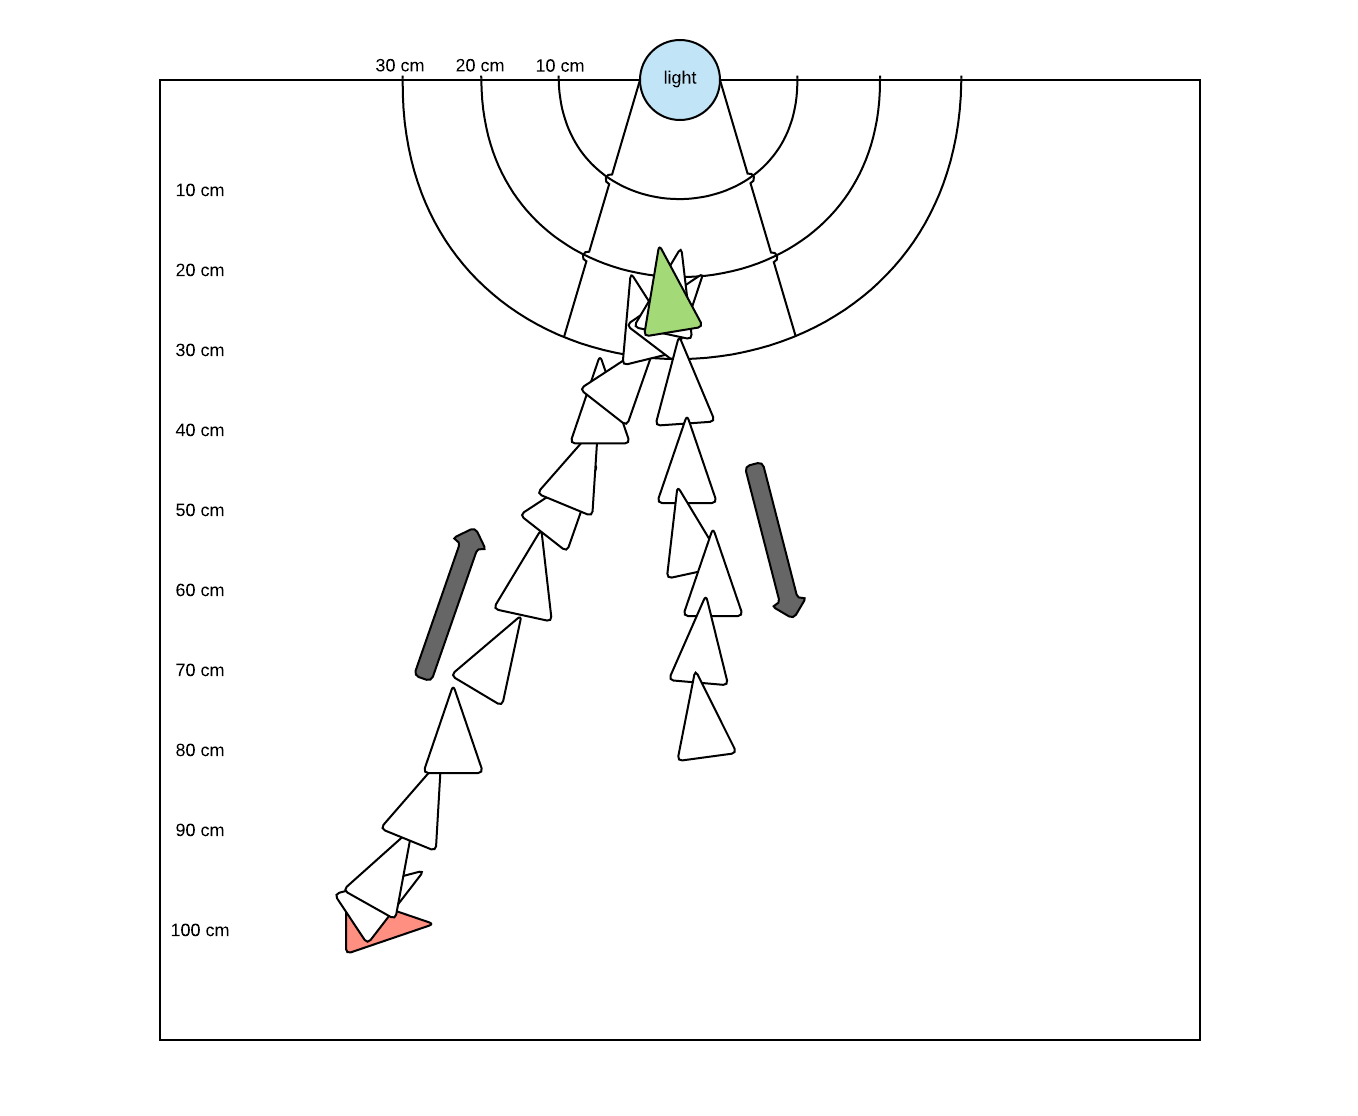
\includegraphics[height=250px]{img/experiment2}
  \caption{Graphical representation of final experiment.}
  \label{fig:experiment}
\end{figure}

Figure \ref{fig:experiment} is a graphical representation of the final experiment, based on the observation and video recording of its proceeding.
The experiment was run multiple times, the figure however only represents a single instance representative of the whole.
In the experiment, the robot starts at approximately $1 m$ distance to the light source, represented by the red triangle.
Its initial behaviour is to follow the light source by always facing in its direction and advance.
The transmitter continuously sends the same message at fixed intervals of 1 second.
At the initial distance, the robot is only able to identify the direction of the source, but is not able to decipher the message.
After several attempts, when the robot gets in range between $20$ and $30 cm$, it is also able to correctly interpret the message.
In the figure, this moment is represented by a green triangle.
In this experiment, the message sent is a negative velocity, that cause the robot to retreat away from the light.
An unexpected behaviour that presented itself multiple times is that once the robot enters an area between $30$ and $50 cm$ from the source and is centred in regards to the source's position, it readjusts its direction more often than usual, hesitating and advancing more slowly.
Due to the narrow angle between the front sensors and the distance from the source, the three front sensors are hit by a comparable intensity of light, causing random noise to dictate one direction in favour of another, multiple times.
When this happens the robot immediately readjusts, and the same happens over and over, causing the robot to slow down its advancement.
This ultimately leads to more time spent in direct sight of the signal, which in turn causes the robot to receive the message at longer distances than expected.

\todo{angle part with multiple sources}









